\chapter{Input/Output Setup}

\section{Overview}
In this chapter, we will discuss various input-output setups (depending on \emph{how many antennas are used in both the transmitter and the receiver}) that were implemented in the simulator. \\
The availability of multiple antennas at the transmitter and/or the receiver can be utilized in different ways to achieve different aims:
\begin{itemize}
    \item Multiple antennas at the transmitter and/or the receiver can be used to provide additional diversity against fading on the radio channel. In this case, the channels experienced by the different antennas should have low mutual correlation, implying the need for a sufficiently large inter-antenna distance (spatial diversity), alternatively the use of different antenna polarization directions (polarization diversity).
    \item Multiple antennas at the transmitter and/or the receiver can be used to “shape” the overall antenna beam (transmit beam and receive beam, respectively) in a certain way, for example, to maximize the overall antenna gain in the direction of the target receiver/transmitter or to suppress specific dominant interfering signals.
    \item The simultaneous availability of multiple antennas at the transmitter and the receiver can be used to create what can be seen as multiple parallel communication “channels” over the radio interface. This provides the possibility for very high bandwidth utilization without a corresponding reduction in power efficiency or, in other words, the possibility for very high data rates within a limited bandwidth without an un-proportionally large degradation in terms of coverage. This feature is highly present in the MIMO setup.
\end{itemize}

The following table explains the different setups implemented in the simulator.
\begin{table}[!ht]
    \centering
    \caption{Transmitter \& Receiver for different setups}
    \label{tbl:mytable}
    \begin{tabular}{lll}
        \toprule
        Setup & Transmitter & Receiver \\
        \midrule
        SISO (Single-Input Single-Output)  & One antenna   & One antenna   \\
        SIMO (Single-Input Multi-Output)   & One antenna   & Many antennas \\
        MISO (Multi-Input Single-Output)   & Many antennas & One antenna   \\
        MIMO (Multi-Input Multi-Output)    & Many antennas & Many antennas \\
        \bottomrule
    \end{tabular}
\end{table}

Later in the chapter we will discuss how each setup works, its encoding and decoding techniques and benifits. We will also zoom in as if we were to send only one symbol. This will help us explain the techniques used in each setup better.

\begin{GrayBox}
    \textbf{Before we discuss each setup in great detail, some information about the channel model must be cleared out:}
    \begin{itemize}
        \item We are using an OFDM based system.
        \item Each sub-carrier carries only one modulated symbol.
        \item We let the channel model be a block fading channel where the channel stays the same for some time (Coherence time) and for some subcarriers (Coherence bandwidth).
    \end{itemize}

    \textbf{The following assumptions were also made:}
    \begin{itemize}
        \item We will ignore the modulation of the input signal for better understanding of how each setup works.
        \item We will also assume perfect knowledge of the channel at both the transmitter and the receiver.
    \end{itemize}
\end{GrayBox}

\subsection{Narrow-band wireless fading channel}
One of the most common wireless channel model and the one that we will be using is the following
\[y[m]=h[m]x[m]+n[m]\]
Where the index m is a time index, $x[m]$ is the transmitted complex symbol at time m, $y[m]$ is the corresponding receives signal, and $n[m]$ is the AWGN at time m.\\
The different component compared to the AWGN channel is $h[m]$. This is referred to as the “fading” coefficient. It is a random value which captures the changes that happen in the transmitted electromagnetic waves due to the environment. \\
$h[m]$ is modelled as a complex number, where
\begin{equation}
    \label{eq:h channel}
    h[m]=\text{a}+j\text{b}= |h[m]| e^{j\theta[m]}
\end{equation}
\begin{wrapfigure}{h}{0.4\textwidth}
    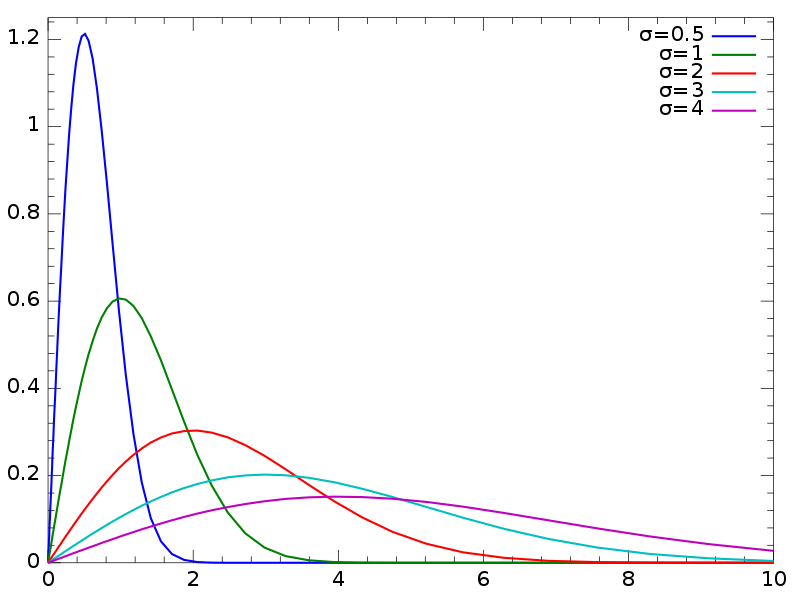
\includegraphics[width=0.4\textwidth]{22.PNG}
  \caption{Rayleigh random variable}
\end{wrapfigure}
where the magnitude of the channel $|h[m]|$ is a Rayleigh random variable
\[|h[m]|  ~ f_{\sigma^2}(x)=\frac{x}{\sigma^2}  e^{\frac{-x^2}{2\sigma^2 }}\]  
The phase $\theta[m]$ is a uniform random variable.
The figure shows a Rayleigh distribution for different values of $\sigma$. This shows the impact of fading on communications. Specifically, the value of $|h[m]|$ can be small with a considerable probability, and that effectively reduces the received power of the transmitted signal. When $|h[m]|$  is too small, the channel is said to be in deep fading. 

\section{SISO}
SISO stands for \textbf{"Single Input, Single Output"}. In communication engineering, SISO is the simplest way to describe a communication link between a transmitter and a receiver. It is used to describe the case where both the transmitter and receiver have single antennas. Pre-coding is not typically used in SISO communication systems. \\
For a SISO channel (we drop the time index for now)
\begin{equation}
    \label{eq:simplest channel model}
    y = hx + n
\end{equation}
The noise power is $N_o$. The minimum distance between Constellation points without fading is $2a$, where $a$ is the smallest transmitted amplitude per constellation points.
Now, with fading coefficient $h$, minimum distance becomes $d_{min}=2|h|a$. There, for this CSI value, we can upper bound the probability of error as
\begin{equation}
    \label{eq:upper bound Pe for SISO}
    P_e\left(\bar{h}\right)\le\ k\ Q\left(\frac{d_{min}}{\sqrt{2N_o}}\right)=\ k\ Q\left(\sqrt{\frac{4\left|h\right|^2a^2}{N_o}}\right)=k\ Q\left(\sqrt{2\left|h\right|^2\text{SNR}}\right)
\end{equation}

We assume that $h$ is Rayleigh (as described in equation~\ref{eq:h channel}) with $\sigma^2= 1$.
Then, we want to compute the "average" $P_e$ over CSI realization. This turns out to be
\begin{equation}
    \label{eq:avg Pe for SISO}
    P_{e\ }=\mathbb{E}_{\left|h\right|^2}\{P_e\left(h\right)\} \le k \left(\frac{1}{2}-\frac{1}{2}\sqrt{\frac{\text{SNR}}{1+\text{SNR}}}\right) =\frac{k}{2}\left(1-\mu\right)
\end{equation}

\textbf{How does this compare with AWGN?} \\
\textbf{Recall:} $P_e$ for AWGN is bounded by $k Q(\sqrt{2\text{SNR}})$. \\
The following figure compares Pe for both AWGN and fading far BPSK.
\begin{figure}[h]
    \centering
    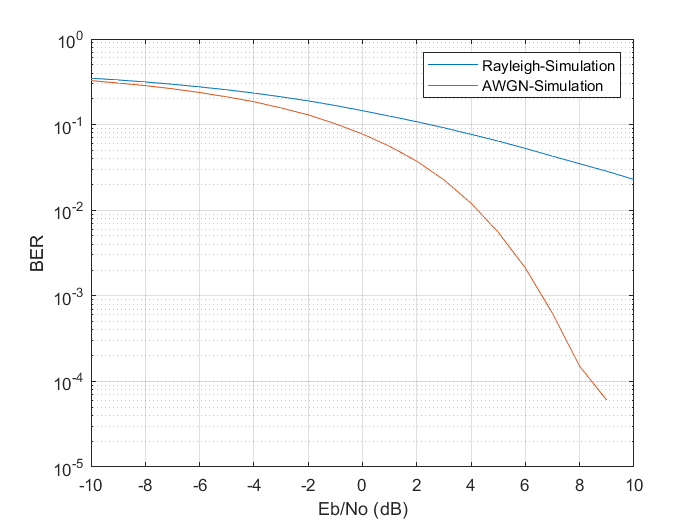
\includegraphics[width=0.7\textwidth]{23.PNG}
    \caption{AWGN vs Rayleigh fading BER for SISO}
    \label{fig:BER SISO}
\end{figure}

At high SNR: \\
Probability of error in AWGN has a water fall behavior which indicates very good performance.
However, it decays linearly in case of fading and that is too slow.
This is because $|h|$ is many times too small and therefore the received power $|h|^2 a^2$ is not enough to make decoding performance good.
we say that a channel in \emph{"deep fade"} if received signal power is less than or equal to the noise power. \\
\[\left|h\right|^2a^2\le N_o\]
\[|h|^2\le \frac{N_o}{a^2}\ =\ \frac{1}{\text{SNR}}\] \\
What is the probability of this happening? \\
This probability is found to can be approximated to 
\begin{equation}
    \label{eq:SISO Pe}
    10\log\left(\mathbb{P}\{|h|^2\le \frac{1}{\text{SNR}}\} \right)= \text{const}-10\log\left(\text{SNR}\right)=\text{const}-\text{SNR}_{dB}
\end{equation}
This looks like the linear decrease behavior we saw above in Figure~\ref{fig:BER SISO}.

\section{SIMO}

\section{MISO}

\section{MIMO}
MIMO stands for \emph{Multiple-In Multiple-Out}, referring to the fact that when a packet is transmitted into the channel it transmitted on more than one antenna and when it comes out of the channel it is received on multiple antennas. This is in contrast to a Single-In Single-Out system with one antenna on both ends of the link, or a SIMO system which would include some types of radios that use diversity combining at the receive end but still transmit over only a single antenna.
\begin{figure}[ht]
    \centering
    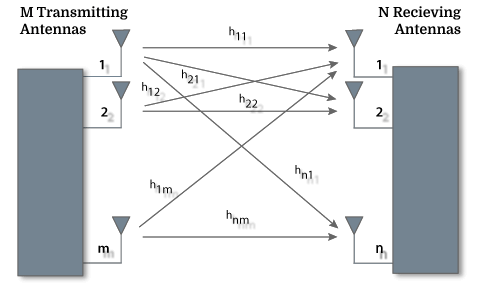
\includegraphics[width=0.5\textwidth]{MIMO.PNG}
    \caption{MIMO Setup}
    \label{fig:MIMO}
\end{figure}

Multiple antennas at the transmitter and receiver introduces signaling degrees of freedom that were absent in SISO systems. This is referred to as the spatial degree of freedom. The spatial degrees of freedom can either be exploited for “diversity” or “multiplexing” (will be discussed later in this chapter in Sec~\ref{subsection:MIMO-Diversity} \& Sec~\ref{subsection:MIMO-Multiplexing}).

\begin{GrayBox}
    \textbf{Alternative View:} \\
    We can think of MIMO as if it were to be a Multi-user MISO system with \emph{one BS} with multiple antennas and \emph{multiple} users with single antennas.
\end{GrayBox}

For any MIMO setup with $m$ transmitting antennas and $n$ receiving antennas (shown in Figure~\ref{fig:MIMO}), the channel model shown in Equation~\ref{eq:simplest channel model} will not hold simply because we have multiple antennas for both Tx and Rx, instead each received symbol $y_i$ is described as:
\begin{equation}
    \label{eq:y_i MIMO}
    y_i = h_{i1} x_1 + h_{i2} x_2 + \ldots + h_{iM} x_M + n_i \qquad \text{for } i=1,\ldots,N
\end{equation}
We can represent the above equation in matrix form for all received symbols $\bar{y}$
\begin{equation}
    \label{eq:y_bar MIMO}
    \bar{y} = \bar{\bar{H}} \bar{x} + \bar{n}
\end{equation}
\[ \text{where}: \quad \bar{y} = \left[ \begin{array}{c}
    y_1 \\
    \vdots \\
    y_N
\end{array} \right] , \bar{\bar{H}} = \left[ \begin{array}{c c c}
    h_{11} & \cdots & h_{1M} \\
    \vdots & h_{ij} & \vdots \\
    h_{N1} & \cdots & h_{NM}
\end{array} \right] , \bar{x} = \left[ \begin{array}{c}
    x_1 \\
    \vdots \\
    x_M
\end{array} \right] , \bar{n} = \left[ \begin{array}{c}
    n_1 \\
    \vdots \\
    n_N     
\end{array} \right] \]
and $\bar{n} \in \mathcal{N} \mathcal{C}\left( 0, N_o \cdot I_{N \times N} \right)$

\subsection{Diversity}
\label{subsection:MIMO-Diversity}
In MIMO diversity, multiple antennas are trying to receive the same signal. The received signal on the two antennas is corrupted by noise that is uncorrelated between antennas, therefore by combining the two signals a better quality signal can be reconstructed. The analogy here is that by looking at the same object from two different vantage points, richer information on the object can be obtained.

\subsubsection{Singular Value Decomposition of Channel}
To achieve this effect, the message must be encoded at the transmitter and decoded at the receiver. This is done with the help of SVD (Theorem~\ref{theo:SVD}).

\newtcbtheorem[auto counter,number within=section]{SVD_theo}
  {Theorem}{fonttitle=\bfseries\upshape, fontupper=\slshape,
     arc=0mm, colback=black!5!white,colframe=black!75!white}{theorem}

\begin{SVD_theo}{Singular Value Decomposition}{}
    For any arbitrary matrix $A \in \mathbb{R}^{m \times n}$ admits a decomposition of the form
    \begin{equation}
        \label{theo:SVD}
        \begin{aligned}
            A &= \sum_{i=1}^{r} \sigma_i u_i v^T_i \\
            &= U \tilde{S} V^T \\
            \tilde{S} &:= \left( \begin{array}{c c}
                S & 0 \\
                0 & 0
            \end{array} \right)
        \end{aligned}
    \end{equation}
    where $U \in \mathbb{R}^{m \times m}$ , $V \in \mathbb{R}^{n \times n}$ are both orthogonal matrices, and the matrix $S$ is a diagonal:
    \[ S = \text{diag}\left( \sigma_1 , \ldots , \sigma_r \right) \]
    where the positive numbers $\sigma_1 \ge \ldots \ge \sigma_r >0$ are unique, and are called the \emph{singular values} of $A$.
    The number $r \leq \min(m,n)$ is equal to the \emph{rank} of $A$, and the triplet $(U,\tilde{{S}},V)$ is called a \emph{singular value decomposition (SVD)} of $A$.
    The first $r$ columns of $U: u_i, i=1,\ldots,r$ (resp. $V: v_i, i=1,\ldots,r$) are called left (resp. right) \emph{singular vectors} of $A$, and satisfy
    \[ Av_i = \sigma_i u_i \quad , \quad u_i^T A = \sigma_i v_i \quad , \quad i = 1,\ldots,r \]

\end{SVD_theo}

Applying SVD to the channel gain matrix $\bar{\bar{H}}$ we get
\begin{equation}
    \label{eq:SVD H}
    \bar{\bar{H}} = \bar{\bar{U}} \bar{\bar{S}} \bar{\bar{V}}^H
\end{equation}
where $\bar{\bar{U}}$ and $\bar{\bar{V}}$ are unitary matrices ($\bar{\bar{U}}^H\bar{\bar{U}} = I$) and $S$ is a diagonal matrix with the singular values of $\bar{\bar{H}}$.
\begin{figure}[ht]
    \centering
    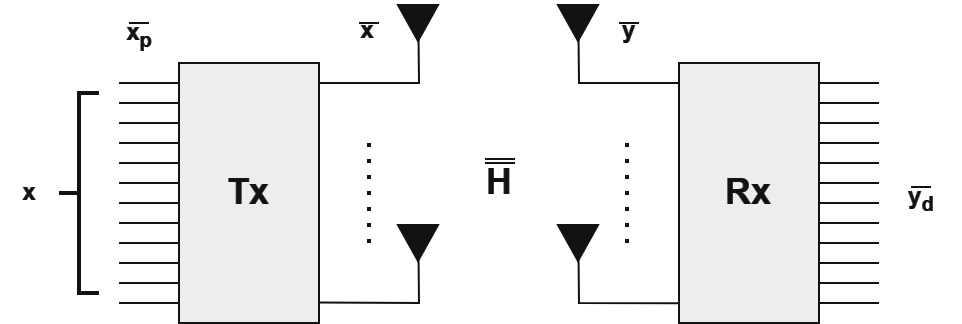
\includegraphics[width=0.65\textwidth]{MIMOdiv.PNG}
    \caption{MIMO setup used for diversity}
    \label{fig:MIMOdiv}
\end{figure}

\subsubsection{Pre-coding at Transmitter}
Now, we will use the decomposition of the channel to pre-code the signal sent at the transmitter. Let $\bar{x_p}$ denotes the raw signal before being sent at the transmitter, then 
\begin{equation}
    \label{eq:pre-coded x}
    \bar{x} = \bar{\bar{V}} \bar{x_p}
\end{equation}
where
\[ \bar{x_p} = \frac{1}{\sqrt{M}} \left[ \begin{array}{c}
    x \\
    \vdots \\
    x
\end{array} \right]_{M \times 1} \]
and $x$ denotes the input message desired to be sent over all the antennas.

\subsubsection{Decoding at Transmitter}
At the receiver, the antennas have received $\bar{y}$ following the channel model in Equation~\ref{eq:y_bar MIMO}. Let $\bar{y_d}$ denotes the decoded received message where $\bar{y_d} = \bar{\bar{U}}^H \bar{y}$.
\begin{equation}
    \label{eq:decoding y_bar}
    \begin{aligned}
        \bar{y_d} &= \bar{\bar{U}}^H \bar{y} \\
        &= \bar{\bar{U}}^H \left[ \bar{\bar{U}} \bar{\bar{S}} \bar{\bar{V}}^H \bar{x} + \bar{n} \right] \\
        &= \bar{\bar{U}}^H \bar{\bar{U}} \bar{\bar{S}} \bar{\bar{V}}^H \bar{x} + \bar{\bar{U}}^H \bar{n} \\
        &= \bar{\bar{U}}^H \bar{\bar{U}} \bar{\bar{S}} \bar{\bar{V}}^H \bar{\bar{V}} \bar{x_p} + \tilde{n} && \text{from \ref{eq:pre-coded x}} \\
        &= \bar{\bar{S}} \bar{x_p} + \tilde{n}
    \end{aligned}
\end{equation}
Therefore by simplifying Equation~\ref{eq:decoding y_bar}, we deduce that each received symbol
\[ y_{d_i} = \sigma_i \frac{1}{\sqrt{M}} x + \tilde{n}_i \]
and the total received signal becomes
\begin{equation}
    \label{eq:y for mimo div}
    \bar{y_d} =  \frac{1}{\sqrt{M}} \left[ \begin{array}{c}
        \sigma_1 \\
        \vdots \\
        \sigma_r
    \end{array} \right] x + \tilde{n}
\end{equation}

This setup yields an improvement in SNR that is equal to $\|H\|_F^2 \cdot \frac{1}{M}$ where
\[\|H\|_F^2 = \sum_{i=1}^{M} \sum_{j=1}^{N} |h_{ij}|^2\]
This improvement is the \emph{diversity gain}, and obtained due to the usage of MIMO system.  
\begin{GrayBox}
    \textbf{Diversity gain} is the increase in signal-to-interference ratio due to some diversity scheme, or how much the transmission power can be reduced when a diversity scheme is introduced, without a performance loss.
\end{GrayBox}

The probability of error in the MIMO setup have an upper bound as follows
\[ P_e \left( \bar{\bar{H}} \right) \leq k Q\left( \sqrt{ 2 \|H\|_F^2 \frac{\text{SNR}}{M} } \right) \] 
We can then calculate the average $Pe$ as follows
\begin{equation}
    \label{eq:avg Pe mimo}
    \begin{aligned}
        P_e &= \mathbb{E}_{\|H\|_F^2} \left\{ P_e \left( \bar{\bar{H}} \right) \right\} \\
        & \leq \text{const.} \cdot \frac{1}{\text{SNR}^{NM}}
    \end{aligned}
\end{equation}
We can see that using MIMO setup also improves $P_e$ of the system drastically.

\subsection{Multiplexing}
\label{subsection:MIMO-Multiplexing}
The second major MIMO technique is Spatial Multiplexing. Spatial multiplexing enables a MIMO transmitter/receiver pair to increase its throughput without increasing bandwidth usage or transmit power. Multiplexing increases throughput linearly with the number of transmit or receive antennas, whichever is lower. The transmitter sends signals carrying different bit streams from each of its antennas. Each receiver antenna receives a linear combination of the transmitted signals.

\subsection{MIMO in Our Simulator}

\subsection{Practical Implementation of MIMO}
All we have talked about so far was under the assumption that both the transmitter and the receiver have perfect knowledge of the channel state at all times. This was a way to ease explaining the concept, but can not be implemented in the simulator.\\
Therefore, we had to implement another way to decode the received signal using $\bar{\bar{U}}$ from the SVD of $\bar{\bar{H}}$ (in Equation~\ref{eq:decoding y_bar}).